\dev{Daphné Kany}{}

\textit{Cette leçon présente le jeu de Nim et ses stratégies gagnantes dans le cas d'une puis plusieurs lignes de bâtons. Les conventions d'écritures sont pour l'instant celles du plan de la leçon sur les jeux.}

\paragraph{I - Jeu de Nim à un tas}

\begin{definition}
	Le jeu de Nim est un jeu à deux joueurs $J_{1}$ et  $J_{2}$. Initialement, on dispose de n bâtons. A tour de rôle, les joueurs retirent au choix 1, 2, ou 3 bâtons. Le joueur qui retire le dernier a gagné. 
\end{definition}

\paragraph{Modélisation : \\}
Soit $G=(V_{1} \sqcup V_{2}, A)$ le graphe représentant un jeu de Nim à n bâtons. \\

$\bullet$ Pour $i \in \{1,2\}, V_{i} = \{(k, i) | k \in \{0,.., n\}\}$ et $G_{i} = \{(0, 3-i)\}$ \\

$\bullet$  $A = \{(k, i) \rightarrow (k', j) | k-k' \in \{1,2,3\}$ et $i \neq j \}$

\begin{example}
	On représente le graphe pour n = 5. \\
	
	\begin{tikzpicture}[->, node distance=2cm]
		\node[state] (q0) {(0,1)};
		\node[state, right of = q0, red] (q1) {(1,1)};
		\node[state, right of = q1, red] (q2) {(2,1)};
		\node[state, right of = q2, red] (q3) {(3,1)};
		\node[state, right of = q3] (q4) {(4,1)};
		\node[state, right of = q4, red] (q5) {(5,1)};
		\node[state, below of = q0, red] (q6) {(0,2)};
		\node[state, right of = q6] (q7) {(1,2)};
		\node[state, right of = q7] (q8) {(2,2)};
		\node[state, right of = q8] (q9) {(3,2)};
		\node[state, right of = q9, red] (q10) {(4,2)};
		\node[state, right of = q10] (q11) {(5,2)};
		\draw (q5) edge[] node{} (q10) ;
		\draw (q5) edge[] node{} (q9) ;
		\draw (q5) edge[] node{} (q8) ;
		\draw (q4) edge[] node{} (q9) ;
		\draw (q4) edge[] node{} (q8) ;
		\draw (q4) edge[] node{} (q7) ;
		\draw (q3) edge[] node{} (q8) ;
		\draw (q3) edge[] node{} (q7) ;
		\draw (q3) edge[] node{} (q6) ;
		\draw (q2) edge[] node{} (q7) ;
		\draw (q2) edge[] node{} (q6) ;
		\draw (q1) edge[] node{} (q6) ;
		\draw (q11) edge[] node{} (q2) ;
		\draw (q11) edge[] node{} (q3) ;
		\draw (q11) edge[] node{} (q4) ;
		\draw (q10) edge[] node{} (q1) ;
		\draw (q10) edge[] node{} (q2) ;
		\draw (q10) edge[] node{} (q3) ;
		\draw (q9) edge[] node{} (q0) ;
		\draw (q9) edge[] node{} (q1) ;
		\draw (q9) edge[] node{} (q2) ;
		\draw (q8) edge[] node{} (q1) ;
		\draw (q8) edge[] node{} (q0) ;
		\draw (q7) edge[] node{} (q0) ;
	\end{tikzpicture}
\end{example}

\paragraph{Calcul de l'attracteur de G1 (positions gagnantes de J1) :}
\enspace\\
$Attr_{0}(G_{1}) = \{(0,2)\}$ \\
$Attr_{1}(G_{1}) = \{(0,2)\} \cup \{u \in V_{2} | N^{+}(u) = (0,2)\} \cup \{u \in V_{1} | (0,2) \in N^{+}(u)\} = \{(0,2), (1,1), (2,1), (3,1)\}$ \\
$Attr_{2}(G_{1}) = \{(0,2), (1,1), (2,1), (3,1), (4,2)\}$ \\
On montre par récurrence : \\
$Attr_{i}(G_{1}) = \{(4*k, 2) | k \le (i-1)\} \cup \{(u, 1) | u$ mod 4 $\neq$ 0 et $u \le 4*i\}$

\paragraph{Conclusion : \\}
$J_{1}$ a une stratégie gagnante ssi (il commence et n mod 4 $\neq$ 0) ou ($J_{2}$ commence et n mod 4 = 0).

\paragraph{II - Jeu de Nim à k tas}

\begin{com}
	On voudrait maintenant généraliser le jeu de Nim : Les joueurs ont devant eux k lignes de bâtons. Ils retirent à tour de rôle un nombre strictement positif de bâtons d'une des lignes. Le joueur qui retire le dernier gagne. 
\end{com}

\begin{proposition}
	Soit un jeu de Nim à k lignes $N_{1}, .. N_{k}$, de position initiale respective $s_{1}$, ..., $s_{k}$. On pose $S = s_{1} \oplus s_{2}\oplus ... \oplus s_{k}$. Alors $J_{1}$ a une stratégie gagnante ssi (il commence et $S > 0$) ou ($J_{2}$ commence et $S = 0$). 
\end{proposition}

\begin{proof}
	\paragraph{Sens indirect : } 
	Soit $P_{i}$ : «Pour une partie de i coups ($J_{1}$ commence et $S > 0$) ou ($J_{2}$ commence et $S = 0$) $\implies$ $J_{1}$ a une stratégie gagnante»\\
	Si i = 0 : Alors l'état initial est (0, .., 0) donc $J_{1}$ gagne si $J_{2}$ commence.\\
	Hérédité : Soit i > 0 tq $P_{i-1}$. Montrons $P_{i}$. \\
	Supposons $J_{1}$ commence et S > 0. Il existe une ligne $N_{l}$ tq le bit de poids fort de S est à 1 dans $s_{l}$. $J_{1}$ retire des bâtons de cette ligne de façon à annuler  S. On se ramène alors à une partie à n-1 coups dans laquelle $J_{2}$ commence et S = 0, donc par HR, $J_{1}$ a une stratégie gagnante. \\
	Supposons $J_{2}$ commence et S = 0. Alors quelque soit le coup joué par $J_{2}$, il modifie un bit d'une ligne et donc la valeur de S qui devient > 0. On se ramène alors à une partie à n-1 coups dans laquelle $J_{1}$ commence et S > 0, donc par HR, $J_{1}$ a une stratégie gagnante. Ce qui prouve la récurrence. \\
	Par ailleurs, toute partie finit (nombre de bâtons total décroît strictement à chaque tour).
	\paragraph{Sens direct : }
	Par contraposée,  $J_{2}$ a une stratégie gagnante donc $J_{1}$ n'en a pas. 
\end{proof}
\begin{center}
	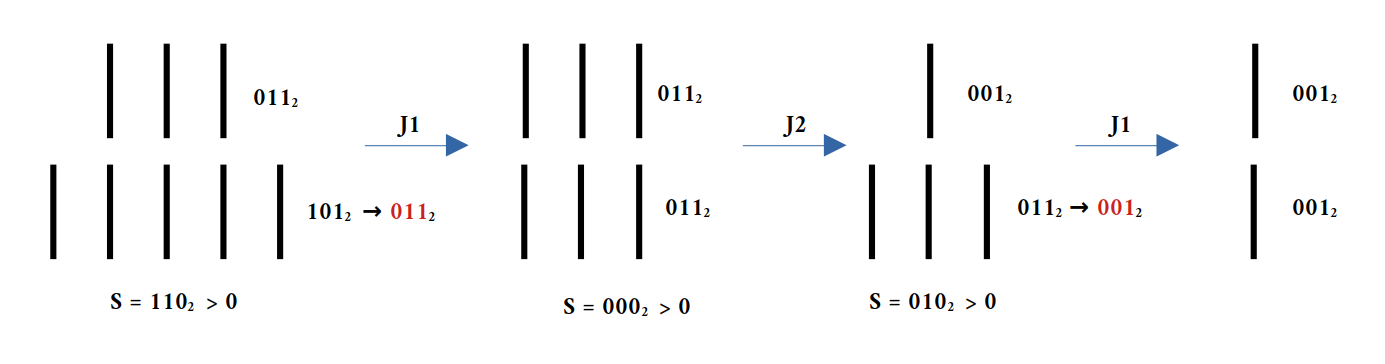
\includegraphics[scale=0.35]{Developpements/Nim/nim.png}
	{Exemple avec deux lignes}
\end{center}
